% Figure from MATH 591 notes, section 67 (the rotation field). Lecture 23 delivery.
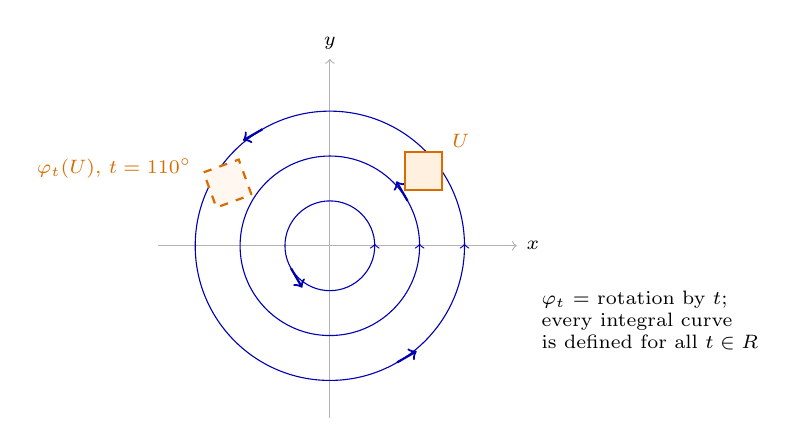
\begin{tikzpicture}[scale=0.95]
\draw[->, gray!60] (-2.3,0) -- (2.5,0) node[right, font=\scriptsize, text=black] {$x$};
\draw[->, gray!60] (0,-2.3) -- (0,2.5) node[above, font=\scriptsize, text=black] {$y$};
\foreach \r in {0.6,1.2,1.8} { \draw[blue!70!black] (0,0) circle (\r); \draw[blue!70!black, ->] (\r,0) ++(0,0.01) -- ++(0,0.02); }
\foreach \a/\r in {30/1.2, 120/1.8, 210/0.6, 300/1.8} { \draw[->, blue!70!black, thick] ({\r*cos(\a)},{\r*sin(\a)}) -- ++({0.3*cos(\a+90)},{0.3*sin(\a+90)}); }
\draw[orange!85!black, thick, fill=orange!12] (1.000,0.750) -- (1.500,0.750) -- (1.500,1.250) -- (1.000,1.250) -- cycle;
\node[orange!85!black, font=\scriptsize] at (1.75,1.4) {$U$};
\draw[orange!85!black, thick, dashed, fill=orange!6] (-1.047,0.683) -- (-1.218,1.153) -- (-1.688,0.982) -- (-1.517,0.512) -- cycle;
\node[orange!85!black, font=\scriptsize, anchor=east] at (-1.72,1.03) {$\varphi_t(U)$, $t = 110^\circ$};
\node[font=\scriptsize, anchor=west, align=left] at (2.7,-1.0) {$\varphi_t$ = rotation by $t$;\\ every integral curve\\ is defined for all $t \in \mathbb{R}$};
\end{tikzpicture}
